\chapter{Theoretical Background on MIR and MER}
\label{chap:TheoreticalBackgroundMIRMER}
\thispagestyle{plain}

\vspace{0.5cm}

\noindent This chapter introduces the readers to the main basics about Music Information Retrieval and Music Emotion Recognition.

\section{Music Information Retrieval}
Music information retrieval (MIR) is the interdisciplinary science of retrieving information from music. MIR is a small but growing field of research with many real-world applications. Those involved in MIR may have a background in musicology, psychoacoustics, psychology, academic music study, signal processing, informatics, machine learning, optical music recognition, computational intelligence or some combination of these.
\\ \indent
MIR is being used by businesses and academics to categorize, manipulate and even create music.
\\
A few application to MIR can be:
\begin{itemize}
	\item Recommended systems: several already exist, but few are based upon MIR techniques, instead making use of similarity between users or laborious data compilation as in \href{https://www.pandora.com}{Pandora}\footnote{https://www.pandora.com}.
	\item Intelligent and adaptive digital audio effects: aim of design a system that determine the settings of audio effects based on the audio content.
	\item Track separation and instrument recognition: like extracting the original tracks as recorded, which could have more than one instrument played per track. Instrument recognition is about identifying the instruments involved into one track.
	\item Automatic music transcription: process of converting an audio recording into symbolic, such score or a MIDI file.
	\item Automatic categorization: common task of MIR is musical genre categorization and is the usual task for the yearly Music Information Retrieval Evaluation eXchange (MIREX).
\end{itemize}

\section{Music Emotion Recognition}
Music Emotion Recognition (MER) aim to research on modeling humans emotion perception of music \cite{yang2011music}, a research topic that emerges in the face of the explosive growth of digital music.
Automatic MER allows users to retrive and organize their music collections in a fashion that is more content-centric than conventional metadata-based methods.
\\
The main challenge is based on the human perception of emotions, their subjective nature of emotion perception. 
Building such a music emotion recognition system, however, is challenging be- cause of the subjective nature of emotion perception. One needs to deal with issues such as the reliability of ground truth data and the difficulty in evaluating the prediction result, which do not exist in other pattern recognition problems such as face recognition and speech recognition. 
\\
MER methods developed try to address the issues related to the ambiguity and granularity of emotion description, the heavy cognitive load of emotion annotation, subjectivity of emotion perception, and the semantic gap between low-level audio signal and high-level emotion perception.

\subsection{Importance of Music Emotion Recognition}
Music plays an important role in human life, even more in the digital age. Never before has such a large collection of music been created and accessed daily by people. Before with the use of compact audio formats with near CD quality such as MP3 and now on with the various streaming services, have greatly contributed to the tremendous growth of digital music libraries.
\\ \indent
Conventionally, the management of music collections is based on catalog metadata, such as artist name, album name, and song title. As the amount of content continues to explode, this conventional approach may be no longer sufficient. The way that music information is organized and retrieved has to evolve to meet the ever increasing demand for easy and effective information access.
\\ \indent
Music, is a complex acoustic and temporal structure, it is rich in content and expressivity. When an individual engages with music as a composer, performer or listener, a very board range of mental processes is involved, including \textit{representational} and \textit{evaluative}. The representational process includes the perception of meter, rhythm, tonality, harmony, melody, form, and style, whereas the evaluative process includes the perception of preference, aesthetic experience, mood, and emotion. The term evaluative is used because such processes are typically both valences and subjective. Both the representational and the evaluative processes of music listening can be leveraged to enhance music retrieval.
According to a study of \href{https://www.last.fm/home}{Last.fm}\footnote{https://www.last.fm/home}, emotion tagging is the third most frequent type of tags (first is genre and second locale) assigned to music pieces by online users.
\\ Even if emotion-based music retrieval was a new idea, a survey conducted in 2004 from \cite{lee2004survey} showed that about 28.2\% of the participants identified emotion as an important criterion in music seeking and organization.
\\ The table \ref{table:browse_music} represent the responses of 427 subjects to the question \textit{"When you search for music or music information, how likely are you to use the following search/browse options?"} \cite{lee2004survey}.
\begin{table}[h!]
\centering
\begin{tabular}{|l | c|}
\hline
Search/Browse by & Positive rate\\ [0.5ex] 
\hline\hline Singer/Performer 			&		96.2\%	\\ 
\hline	Title of work(s) 					& 		91.6\%	\\ 
\hline	Some words of the lyrics 	& 		74.0\% 	\\
\hline	Music style/genre 				&		62.7\%	\\
\hline	Reccomendations 				&		62.2\%	\\
\hline	Similar artist(s)					&		59.3\%	\\
\hline	Similar music 					&		54.2\%	\\
\hline	Associated usage				&		41.9\% 	\\
\hline	Singing								&		34.8\% 	\\
\hline	Theme(main subject)			&		33.4\% 	\\
\hline	Popularity							&		31.0\% 	\\
\hline	\textbf{Mood/emotional state	}	&		\textbf{28.2\%} 	\\
\hline	Time period						&		23.8\% 	\\
\hline	Occasions to use				&		23.6\% 	\\
\hline	Instrument(s)					&		20.8\% 	\\
\hline	Place/event where heard	&		20.7\% 	\\
\hline	Storyline of music			&		17.9\% 	\\
\hline	Tempo								&		14.2\% 	\\
\hline	Record label						&		11.7\% 	\\
\hline	Publisher							&		6.0\% 	\\
\hline
\end{tabular}
\caption{Responses of 427 subjects to the question \textit{"When you search for music or music information, how likely are you to use the following search/browse options?"}}
\label{table:browse_music}
\end{table}

Into another survey \cite{juslin2004expression}, they present findings from an exploratory questionnaire study featuring 141 music listeners (between 17 and 74 years of age) that offers some novel insights.
\\ 
One of the most exciting but difficult endeavors in research on music is to understand how listeners respond to music. It has often been suggested that a great deal of the attraction of music comes from its “emotional powers”. That is, people tend to value music because it expresses and induces emotions.
The table  \ref{table:motivation_music} tries to resume the motivations to the answer \textit{"Why do we listen to music?"}
\begin{table}[h!]
\centering
\begin{tabular}{|l | c|}
\hline
Motive & Ratio\\ [0.5ex] 
\hline\hline "To express, release and influence emotions"	&	47\%	\\ 
\hline "To relax and settle down"										&	33\%	\\
\hline "For enjoyment, fun, and pleasure"							&	22\%	\\
\hline "As company and background sound"						&	16\%	\\
\hline "Because it makes me feel good"								&	13\%	\\
\hline "Because it's a basic need, I can't live without it"		&	12\%	\\
\hline "Because I like, love music"										&	11\%	\\
\hline "To get energized"													&	9\%	\\
\hline "To evoke memories"												&	4\%	\\ 
\hline
\end{tabular}
\caption{Responses of 141 subjects to the question \textit{"Why do you listen to music?"}}
\label{table:motivation_music}
\end{table}

\indent
Some music companies, like  \href{https://www.allmusic.com/moods}{Allmusic.com}\footnote{https://www.allmusic.com/moods}, gives the possibility to search music by emotion labels. With these, the user can retrive and browse artists or albums by emotion.
\\ \indent
Making computers capable of recognizing the emotion of music also enhances the way humans and computers interact. It is possible to play back music that matches the users mood detected from physiological, prosodic, or facial cues. A cellular phone equipped with automatic music emotion recognition (MER) function can then play a song best suited to the emotional state of the user; a smart space (e.g., restaurant, conference room, residence) can play background music best suited the people inside it.

\subsection{Recognizing the perceived emotion of music}
There is a relationship between music and emotions, that has been the subject of much discussion and research in many different disciplines, like philosophy, musicology, sociology.
\\
In psychological studies, emotion are often divided into three categories:
\begin{itemize}
	\item \textit{Expressed emotion}: the ones the performer tries to communicate with the listener.
	\item \textit{\textbf{Perceived emotion}}: represented by music and perceived by the listener.
	\item \textit{Felt or Evoked emotion}: induced by music and felt by the listener.
\end{itemize}

MER focus on perceived emotions because they are less subjective than felt emotions and are often easier to conceptualize. This because felt emotions depends on personal factors and the situation in which the listener processes the song.
From an engineering point of view, one of the main interests is to develop a computational model of music emotion and to facilitate emotion-based music retrieval and organization. MIR community has made many efforts for automatic recognition of the perceived emotion of music, various implementations will be presented further in chapter \ref{chap:StateOfTheArt}.
\\
A typical approach to MER categorizes emotions into a number of classes and applies Machine Learning (ML) techniques to train a classifies. Usually are extracted some features of music to represent the acoustic property of a music piece. Typically, a subjective test is conducted to collect the ground truth needed for training the computational model of emotion prediction. Subjects are asked to report their emotion perceptions of the music pieces.
\\
To learn the relationship between music features and emotion labels have been applied, such as Support Vector Machines (SVMs), Gaussian Mixture Models (GMMs), Neural Networks (NN) and k-nearest neighbor.
\\
After training, the automatic model can be applied to classify the emotion of an input music piece, for example a schematic diagram of the \textit{categorical approach} to MER can be seen in figure \ref{fig:MER_categorical_approach}.

\begin{figure}[h]
    \centering
    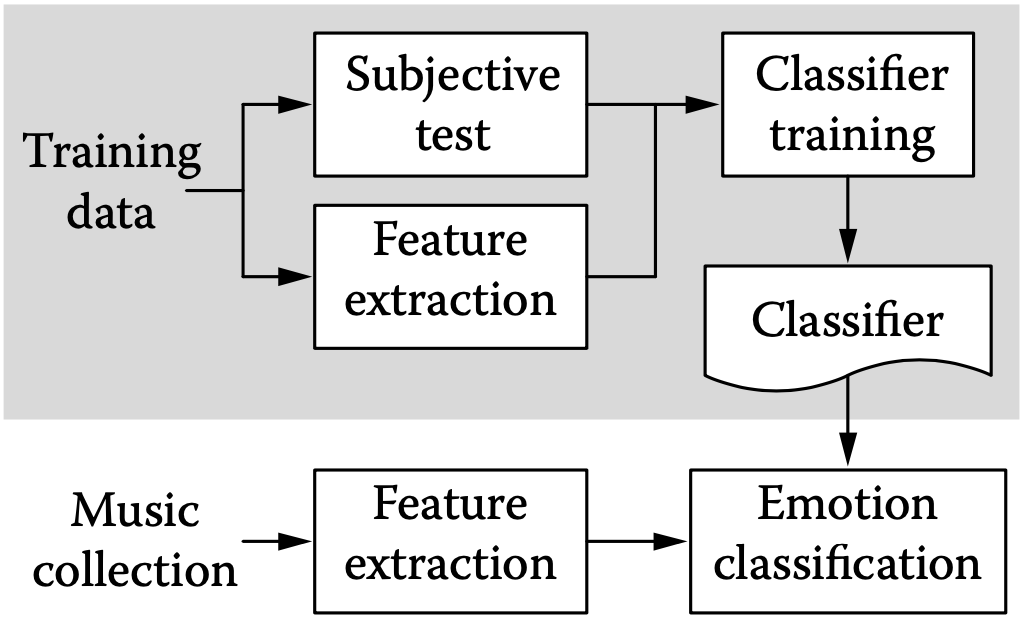
\includegraphics[scale=0.5]{MER_categorical_approach.png} 
	\caption{Schematic diagram of the categorical approach to MER}
    \label{fig:MER_categorical_approach}
\end{figure}

\subsection{Open issues of Music Emotion Recognition} \label{issues}
As MER is a quite new domain, there are some elements that have no clear answer. Four of these issues are:
\begin{enumerate}
	\item Ambiguity and Granularity of emotion description: issue related to the relationship between emotions and the affective terms that denote emotions and the problem of choosing which and how many affective terms to be included in the taxonomy. Emotions are fuzzy concepts, there are main synonyms and similarities between different terms. In general, classification accuracy of an automatic model is inversely proportional to the number of classes considered \cite{van2006emotion}.
	\item Heavy cognitive load of emotion annotation: to collect data for training an automatic model, is typically conducted a subjective test by inviting human subjects to annotate the emotion of music pieces. The problem is that to reduce administrative effort, each music piece is annotated by two or three musical \textit{experts} to gain consensus of the annotation result. Everyday contexts in which musical experts experience is so different from those non-experts require separate treatment. Since MER system is expected to be used in the everyday context, the emotion annotation should be carried out by \textit{ordinary people}.
	\item Subjectivity of emotional perception: music perception is intrinsically subjective and is under the influence of many factors such as cultural background, age, gender, personality and so forth. Therefore conventional categorical approaches that simply assign one emotion class to each music piece in a deterministic manner do not perform very well in practice.
	\item Semantic gap between Low-Level (LL) and audio signal and High Level (HL) Human perception: it is difficult to accurately compute emotion values, and what intrinsic element of music causes a listener to create a specific emotional perception is still far from well understood.
\end{enumerate}

\subsection{Emotion description}
Many researchers have suggested that music is an excellent medium for studying emotion, because people tend to make judgments about music and their affective responses to music.
\\
Music represent emotions that are perceived by the listener or induced emotions that are felt by the listener. Now we will focus on the emotion conceptualization alone, since it's central to have a theoretical background to apply then to MER.
\\
The celebrated paper of Hevner \cite{hevner1935expression} , studied the relationship between music and emotions though experiments where subjects are asked to report some adjectives that came to their mind as the most representative part of a music played. From this have been proposed a large variety of emotion models, like the one presented and used in this thesis.
\\ \indent
The idea of emotion conceptualization is to divide in two different approaches, the \textbf{Categorical approach} and the \textbf{Dimensional approach}.

\paragraph{Categorical approach}
\mbox{} \\ \\ \indent
The first assumption of this emotion conceptualization is that emotions are categorized and categories are distinct from each other. For this approach, there is the idea that there are a limited number of innate and universal emotion categories such as:
\begin{itemize}
	\item Happiness
	\item Sadness
	\item Anger
	\item Fear
	\item Disgust
	\item Surprise
\end{itemize}
All other emotions can be derived from these "\textit{basic emotions}".
\\
In psychological studies, different researchers have come up with different sets of basic emotions.
\\
For example, another famous categorical approach to emotion conceptualization is Hevner's adjective checklist. He found eight clusters positioned in circle as in figure \ref{fig:Hevner_clusters}. The adjective within a cluster are similar, neighbor clusters varies in a cumulative way until reaching the opposite position where there is the contrast cluster. 
\begin{figure}[h]
    \centering
    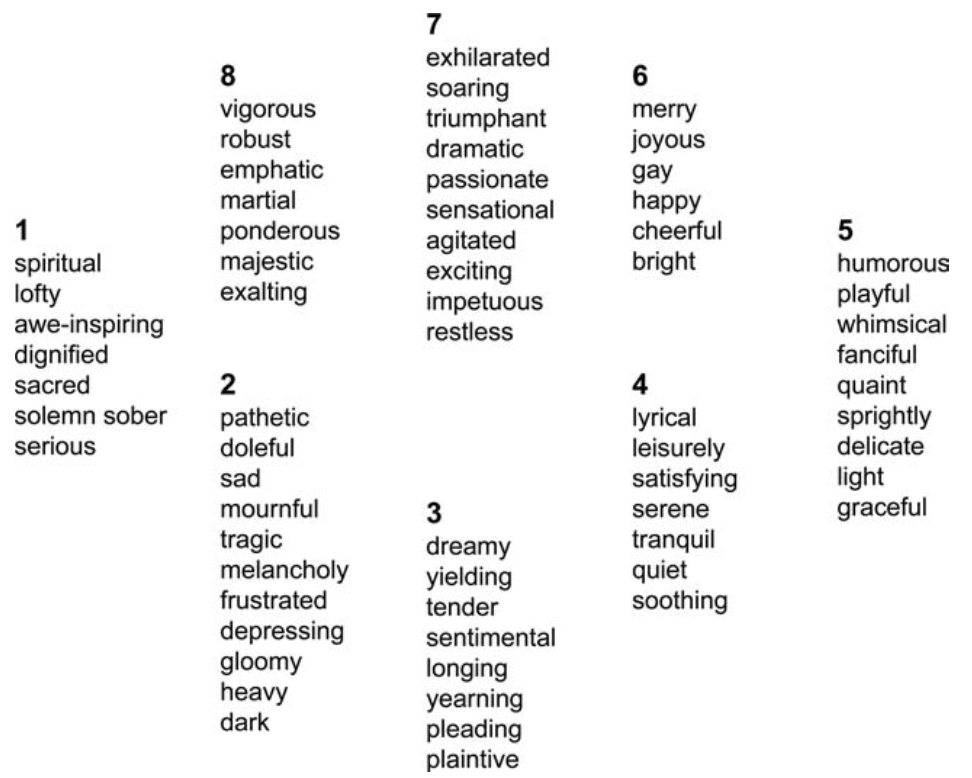
\includegraphics[scale=0.5]{Hevner_clusters.png} 
	\caption{Eight clusters proposed by Hevner}
    \label{fig:Hevner_clusters}
\end{figure}
Hevner's checklist proposed in 1935 was suddenly updated and regrouped into ten groups by Fansworth and into nine groups in 2003 by Schubert.
\\ \indent
Drawbacks of categorical approach is that the number of primary emotion classes is very small in comparison with the richness of music emotion perceived by humans. The problem is in the sense that using a finer granularity, does not necessarily solve the problem because the language for describing emotions is inherently ambiguous and varies from person to person. Using a large number of emotion classes could submerge the subject and is impractical for psychological studies falsing results.

\paragraph{Dimensional approach}
\mbox{} \\ \\ \indent
Categorical approach focuses mainly on the characteristics that distinguish emotions from one another, dimensional approach focuses on identifying emotions based on their position on a small number of emotion "dimensions" called axes, intended to correspond to internal human representation of emotion. These internal emotion dimensions are found by analyzing the correlation between affective terms.
\\ \indent
There are several different names from past researchers gave very similar interpretations of the resulting factors like tension/energy, intensity/softness, tension/relaxation for example. Most of the factors correspond to the two dimensions of emotion the \textit{valence} (positive and negative affective states) and \textit{arousal} (energy and stimulation level).
\\
Russel, proposed a circumplex model of emotion in \cite{russell1980circumplex} which consist in a two-dimensional, circular structure as in figure \ref{fig:Russel_va_model} involving the dimensions of valence and arousal. In this structure, emotions that are inversely correlated, are placed across the circle from one another.
\begin{figure}[h]
    \centering
    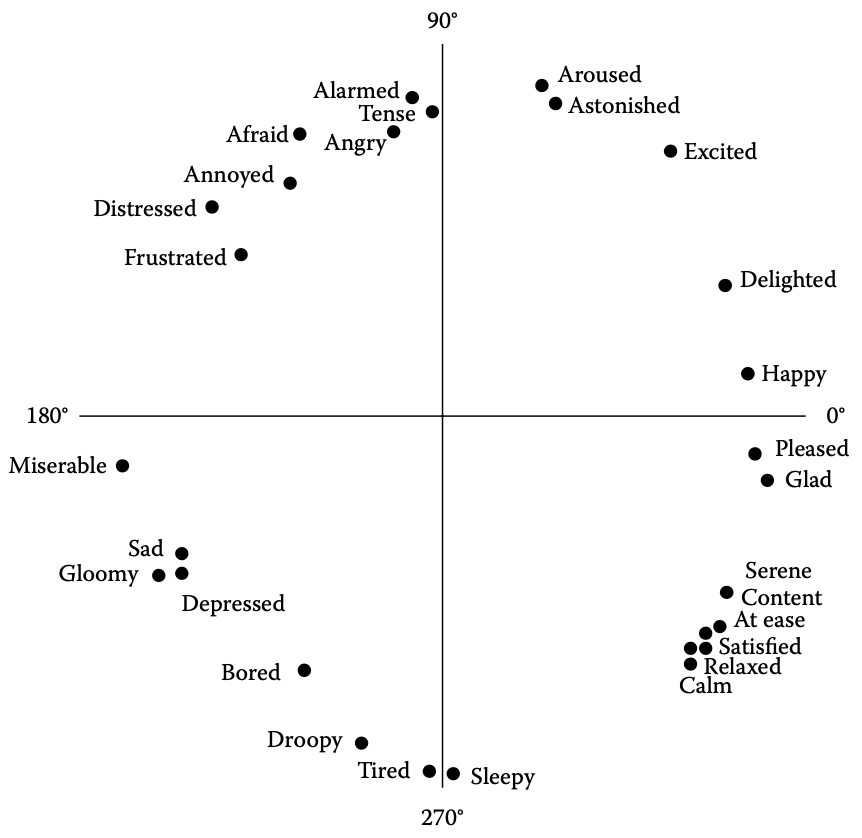
\includegraphics[scale=0.5]{Russel_va_model.png} 
	\caption{Russel's circumplex model of affect}
    \label{fig:Russel_va_model}
\end{figure}

Emotions that are easy to be confused, such as calm and sadness, appear to have similar valence and arousal values. This result implies that valence and arousal may be the most fundamental and most clearly communicated emotion dimensions among others.
Also dimensional approach have its throwbacks, it is argued that dimensional approach blurs important psychological distinctions and consequently obscure important aspects of the emotion process. One example in support of this argumentation is that anger and fear are placed close in the valence-arousal plane but they have very different implications for the organism. Also, it has been argued that using only a few emotion dimension cannot describe all the emotions without residuum.
\\ \indent
Some researches, to overcome to these problems, tries to add a third dimension, called \textit{potency} as dominant/submissive, to obtain a more complete picture of emotion. However, this would increase the cognitive load on the subjects at the same time, requires a more complex interface and makes hard to annotate the process. The third dimension problem is still in discussion.

\paragraph{Music Emotion Variation Detection}
\mbox{} \\ \\ \indent
An important aspect that is not addressed in the previous two paragraphs is the temporal dynamics. Most researches has focused on music piece that are homogeneous with respect to the emotional plane. However, music can change its emotional expression during the song, becomes important to investigate the time-varying relationship between music and emotion. Here is more useful the dimensional approach to capture the continuous changes of emotional expression. Usually subjects are asked to rate valence and arousal in response of the stimulus every second.
\\
For example, songs can be described by valence and arousal curves as in the following figure:
\begin{figure}[h]
    \centering
    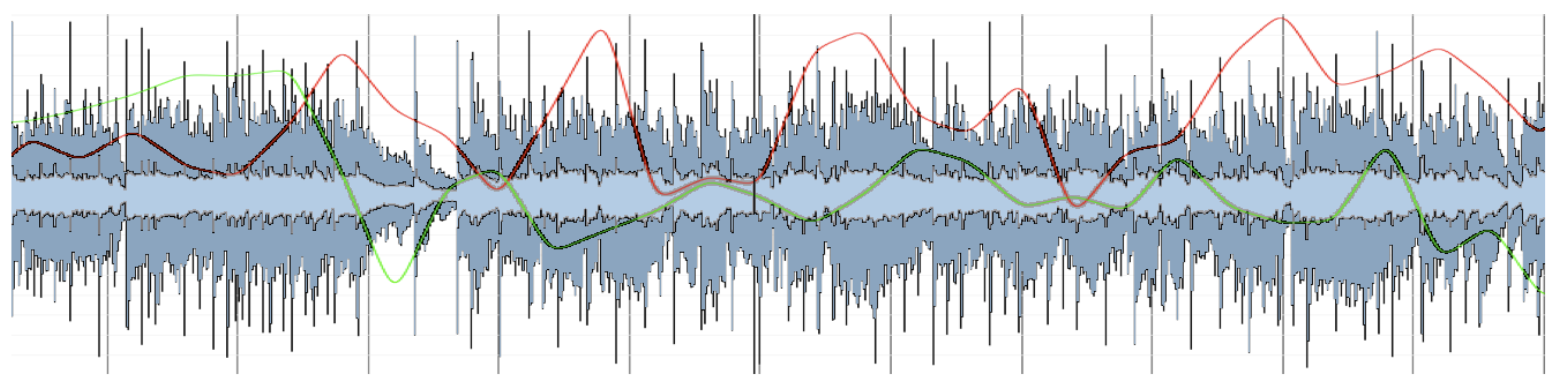
\includegraphics[width=\textwidth]{va_curves.png} 
	\caption{Valence and arousal curves for MEVD}
    \label{fig:va_curves}
\end{figure}

\subsection{Emotion recognition}
MIR researches have been made to automate MER tasks, and the type of music under study has gradually shifted over the past few years from symbolic music to raw audio signal, from Western classical music to popular music. The purpose of MER is to facilitate music retrieval and management in the everyday music listening.
\\ \indent
Nowdays are applied several machine learning techniques to recognize emotion from the music, and the training and automatic recognition model typically consists of the following steps:
\begin{enumerate}
	\item Extract a certain number of features from audio signals to represent the music signal.
	\item Collect from human annotators the ground truth emotion labels or emotion values.
	\item Apply a learning algorithm between music features and emotion labels/values.
	\item Predict emotion of an input song from the resulting computational model.
\end{enumerate}
The music emotion recognition process can be schematized in the figure from \cite{yang2018review}:
\begin{figure}[h]
    \centering
    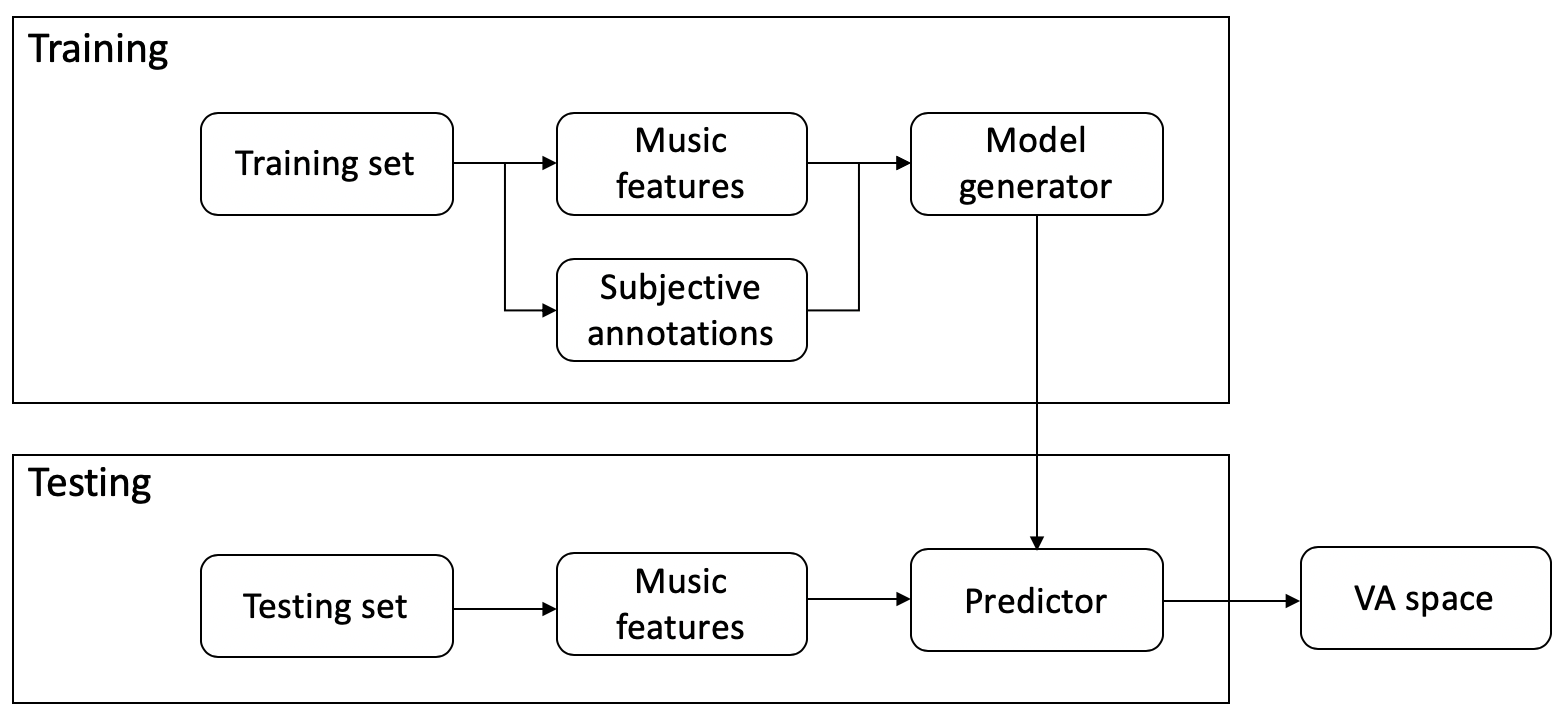
\includegraphics[scale=0.5]{MER_process.png} 
	\caption{MER process}
    \label{fig:MER_process}
\end{figure}
\\
Researches that work on MER can be classified into three approaches.
\\ \indent
The \textbf{categorical approach} that categorizes emotions into a number of discrete classes and applies machine learning techniques to train a classifier. The predicted emotion labels can be incorporated into a text-based or metadata-based music retrieval system.
\\ \indent
The \textbf{dimensional approach} to MER defines emotions as numerical values over a number of emotion dimensions (valence and arousal). A regression model is trained to predict the emotion values that represent the affective content of a song, thereby representing the song as a point in an emotion space. Users can then organize, browse, and retrieve music pieces in the emotion space, which provides a simple means for user interface.

\paragraph{Categorical approach}
\mbox{} \\ \\ \indent
Advantage of categorical approach is that it is easy to be incorporated into a text-based or metadata-based retrieval system. Emotion labels provide an atomic description of music that allows users to retrieve music through a few keywords. Here are present the issues discussed in chapter \ref{issues}.
The commonly adopted methods follows these points:
\begin{enumerate}
	\item Data collection: nowadays there are several large-scale dataset covering all sort of music types and genres. Otherwise is desirable to collect data of the different types, getting rid of the effects called "\textit{album effect}" or "\textit{artist effect}" and collect a variety of music pieces. One problem is that there is no consensus on which emotion model or how many emotion categories should be used. Comparing systems that use different emotion categories  and different dataset is impossible. However the issue concerning how many and which emotion classes should be used seem to remain open.
	\item Data preprocessing: to compare music pieces fairly, music pieces are normally converted to a standard format, and since a complete music piece can contain sections with different emotions,a 20 to 30 second segment is often selected, which is representative of the song (like the chorus part). A good remark of the segment length can be found in \cite{macdorman2007automatic}.
	\item Subjective test: emotion is a subjective matter, so the collection of the ground truth data should be conducted carefully. Annotation methods can be grouped into two categories:
	\begin{itemize}
		\item Expert-based method: which employs a few musical experts to annotate emotions.
		\item Subject-based method: employs a large number of untrained subjects to annotate emotions.
	\end{itemize}
	The ground truth is set by averaging the opinion of all subjects (typically more than 10 subjects per song).
	\\
	It became important to not make a long test, in order to not compromise the reliability of the emotion annotations. Nowadays is introduced the use of listening games.
	\item Features extraction: a certain number of features are extracted from the music signal to represent the different dimension of music listening like melody, timbre and rhythm.
	\\ After features extraction, is applied feature normalization, in order to 
	\item Model training: the following step is to train a Machine Learning (ML) model to learn the relationship between emotion and music. Music emotion classification is carried out with classification ML algorithms, such as Neural Network, k-nearest neighbor (kNN), decision tree, Support Vector Machine (SVM) and Support Vector Classification (SVC).
\end{enumerate}

\paragraph{Dimensional approach}
\mbox{} \\ \\ \indent
The attractive part of dimensional approach is the valence-arousal plane and the associated emotion-based retrieval methods. Due to the fact that the emotion plane contain an infinite number of emotion descriptions, the granularity and ambiguity issues are relieved.
\\
Dimensional perspective is adopted to track the emotion variation of a classical song. The idea of representing the overall emotion of a popular song as a point in the emotion plane for music retrieval, under the assumption that the dominant emotion of a popular song undergoes less changes than a classical song. MER problem became a regression problem, and two independent models, called regressors, are trained to predict the valence-arousal values.
\\
The dimensional approach requires the subjects to annotate the numerical valence-arousal values. This requirement impose an high cognitive load on the subjects.
\\ \\
Pros and cons of categorical and dimensional approach are schematized in the following table:
\begin{table}[h!]
	\centering
	\begin{tabular}{|c|p{0.35\textwidth}|p{0.35\textwidth}|}
	\hline
	& Pros & Cons\\ [0.5ex] 
	\hline\hline Categorical & Intuitive \newline Natural language \newline Atomic description & Lack a unifying model \newline Ambiguous \newline Subjective \newline Difficult to offer fine-grained differentiation \\
	\hline Dimensional & Focus on a few dimensions \newline Good user interface & Less intuitive \newline Semantic loss in projection \newline Difficult to obtain ground truth \\
	\hline
	\end{tabular}
	\caption{Pros and cons of categorical and dimensional approaches}
	\label{table:pros_cons_categorical_dimensional}
\end{table}

\subsection{Valence and Arousal}
As already mentioned before, the valence-arousal plane is the most used dimension plane to represent emotion.
\\
In general, emotional experiences can be described by these two terms, \textit{valence} (positive or negative affectivity) and \textit{arousal} (calming or exciting). Some studies found that valence as well as intensity, is triggered by the amygdala, while the arousal by the reptilian brain.
\\
The common framework for dealing with emotional experience is characterized in a two-dimensional space. Valence ranges from highly negative to highly positive, and arousal ranges from calming/soothing to exciting/agitating:
\begin{figure}[h]
    \centering
    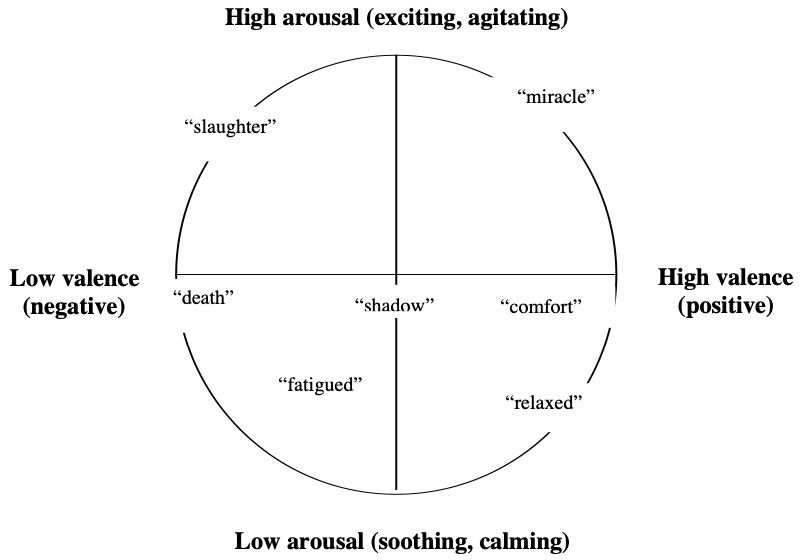
\includegraphics[scale=0.75]{va_plane.png} 
	\caption{Valence and arousal plane, described in \cite{kensinger2004remembering}}
    \label{fig:va_plane}
\end{figure}
High arousal emotional events are encoded better that non-arousing events. Instead of increasing overall attention to an event, an emotionally arousing stimulus decreased attentional resources available for information processing and focused attention only on the arousal-eliciting stimulus.
\\ \indent
The experience of music listening is multidimensional. Different emotions are associated with different music patterns. For example, arousal is associated to:
\begin{itemize}
	\item tempo (fast/slow)
	\item pitch (high/low)
	\item loudness (high/low)
	\item timbre (bright/soft)
\end{itemize}
while valence is associated to:
\begin{itemize}
	\item mode (major/minor)
	\item harmony (consonant/dissonant)
\end{itemize}
as expressed in \cite{gabrielsson2001influence}. Emotion perception is correlated to the combination of music factor, rarely from just one of them. For example, loud chords and high-pitched chords tends to be feel as more positive valence than soft chords and low-pitched chords.

\subsection{Music features}
In MER analysis, an important step to define audio signals is to extract audio features and than apply a feature selection method.
\\
There are several features that can be extracted from audio signal in order to represent five of the most useful perceptual dimensions of music listening:
\begin{itemize}
	\item Energy: dynamic loudness, audio power, total loudness, specific loudness sensation coefficients.
	\item Rhythm: beat histogram, rhythm pattern, rhythm regularity, rhythm clarity, average onset frequency, average tempo.
	\item Temporal: zero-crossing, temporal centroid, log-attack-time.
	\item Spectrum: spectral centroid, spectral rolloff, spectral flux, spectral flatness.
	\item Harmony: salient pitch, chromagram centroid, harmonic change, pitch histogram.
\end{itemize}
These features are just an example of an infinite series of features that can be extracted from audio signals.
\\ \indent
Gabrielsson et al. \cite{gabrielsson2001influence} noted that there are corresponding relations between the dimensional models and music features. Among these features, intensity is a basic feature, which is highly correlated with arousal and is used to classify the arousal dimension \cite{zhang2017feature}.
\\
Nowadays is not really clear the relationship between low-level and mid-level features and mood. In order to capture different aspects is extracted a large set of features. This create a feature matrix that is then normalized in order to map them on the same range of values.
\\ \indent
After the feature matrix is created is applied a feature selection or feature reduction algorithm to select the best set of features. Feature selection algorithms are based on two different ideas:
\begin{itemize}
	\item High-level point of view: find the set of features that best model the concept. This lead to the accuracy of machine learning techniques being limited because of the limitation of the hypothesis done.
	\item Low level point of view: find the set of features that produces the best classification rate.
\end{itemize}
From the machine learning point of view, features are not necessarily of equal importance or quality, and irrelevant or redundant features may lead to inaccurate conclusion. Experiments have shown that, although the performance can thus be improved to a certain extent, using too many features leads to performance degradation \cite{zhang2017feature}.
\\
With an highly discriminant sets of features, is not true that their combination produces a better discriminant power, for example if the set of features is 60, the number of possible combinations are:
\begin{equation}
	n_{combinations} = \sum_{n=1}^{60} \binom{60}{k}
\end{equation}
which is clearly impossible to compute, for this reason is applied some feature selection algorithms.
\\ \indent
An example of feature selection for the categorical approach is the Sequential Feature Selection. It starts from an initial condition, and features are added or removed from a candidate subset while evaluating the \textit{criterion} in two possibilities:
\begin{enumerate}
	\item Sequential Forward Selection (SFS): features are sequentially added to an empty candidate set until the addition of further features does not decrease the criterion.
	\item Sequential Backward Selection (SBS): features are sequentially removed from a full candidate set until the removal of further features increases the chosen criterion.
\end{enumerate}
Another feature selection method is the Minimum-Redundancy-Maximum-Relevance (mRMR) which select the features with the highest relevance to the target class. Relevance is characterized in terms of \textit{mutual information} which is defined as (given $X$ and $Y$ a pair of random variables):
\begin{equation}
	I(x,y)=\iint p(x,y) \log\dfrac{p(x,y)}{p(x)p(y)} dxdy
\end{equation}
where $p(x,y$ is the joint probability mass function of $X$ and $Y$, $p(x)$ and $p(y)$ are the marginal probability mass function of $X$ and $Y$ respectively.
\\ \indent
On the other side, for dimensional approach, feature selection is for example RReliefF \cite{robnik2003theoretical}. Basic idea of this algorithm is that try to estimate the quality of each attribute (in this context the features) according to how well their values distinguish between instances that are close each other.
\\ \indent
Another feature selection for dimensional approach is Principal Component Analysis (PCA) and Independent Component Analysis (ICA). The method starts with all features and reduces them one by one, and hence is similar to backward selection. The goal of ICA is to find a linear representation of non-gaussian data so that the components are statistically independent, or as independent as possible. While the other well known linear transformation methods ( PCA) benefit from the gaussianity of the data, ICA improves the classifier performance in the opposite case.

\subsection{Machine learning}


